\chapter{Simulation in LTspice}

\section{Modeling the Helmholtz Coil}


\begin{figure}[h]
    \centering
    \begin{circuitikz} \draw
        (0,0) to[square voltage source, l=0-5V] (0,4)
        to[R, l=$10\Omega$] (4,4) 
        to[L, l=0.76mH] (4,2) 
        to[L, l=0.76mH] (4,0) -- (0,0)
        ;
    \end{circuitikz}
    \caption{Helmholtz Coil Circuit Diagram}
\end{figure}

Designed the coil in LTspice and simulated the following netlist:

\begin{lstlisting}
    * Helmholtz Coil Simulation
    V1 N001 0 PULSE(0 5 0 {t_edge} {t_edge} {1/2/freq-t_edge} {1/freq})
    R1 VL1 N001 10
    L1 VL1 P001 0.76m
    L2 P001 0 0.76m
    .tran 0 10m 0 1u
    .param t_edge=1u freq=666
    .ic V(VL1)=0
    .backanno
    .end
\end{lstlisting}

\newpage{}
\thispagestyle{plain}

\section{Frequency Analysis}
\subsubsection{T=10L/R $\implies$ f=666Hz}

\begin{figure}[h]
    \centering
    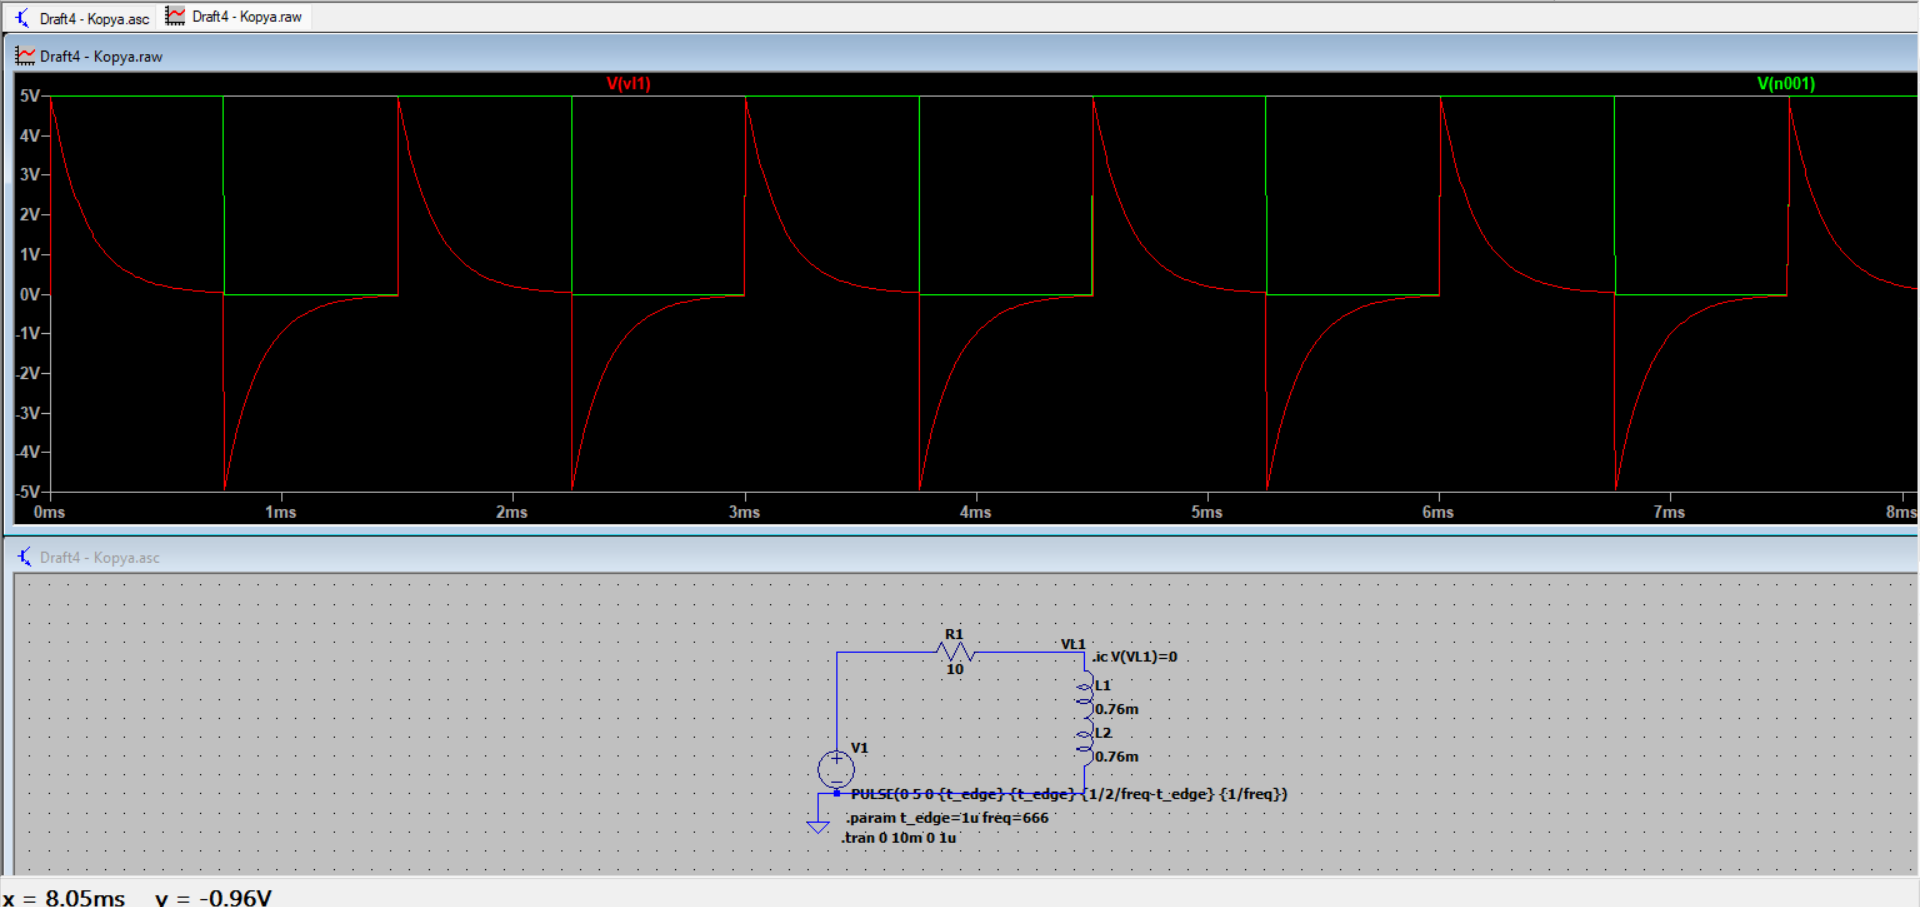
\includegraphics[width=1\textwidth]{assets/666-hz-5vpp-sim.png}
    \caption{666Hz Output @ $5V_{pp}$}
    \label{fig:666-hz-5vpp-output}
\end{figure}

\begin{figure}[h]
    \centering
    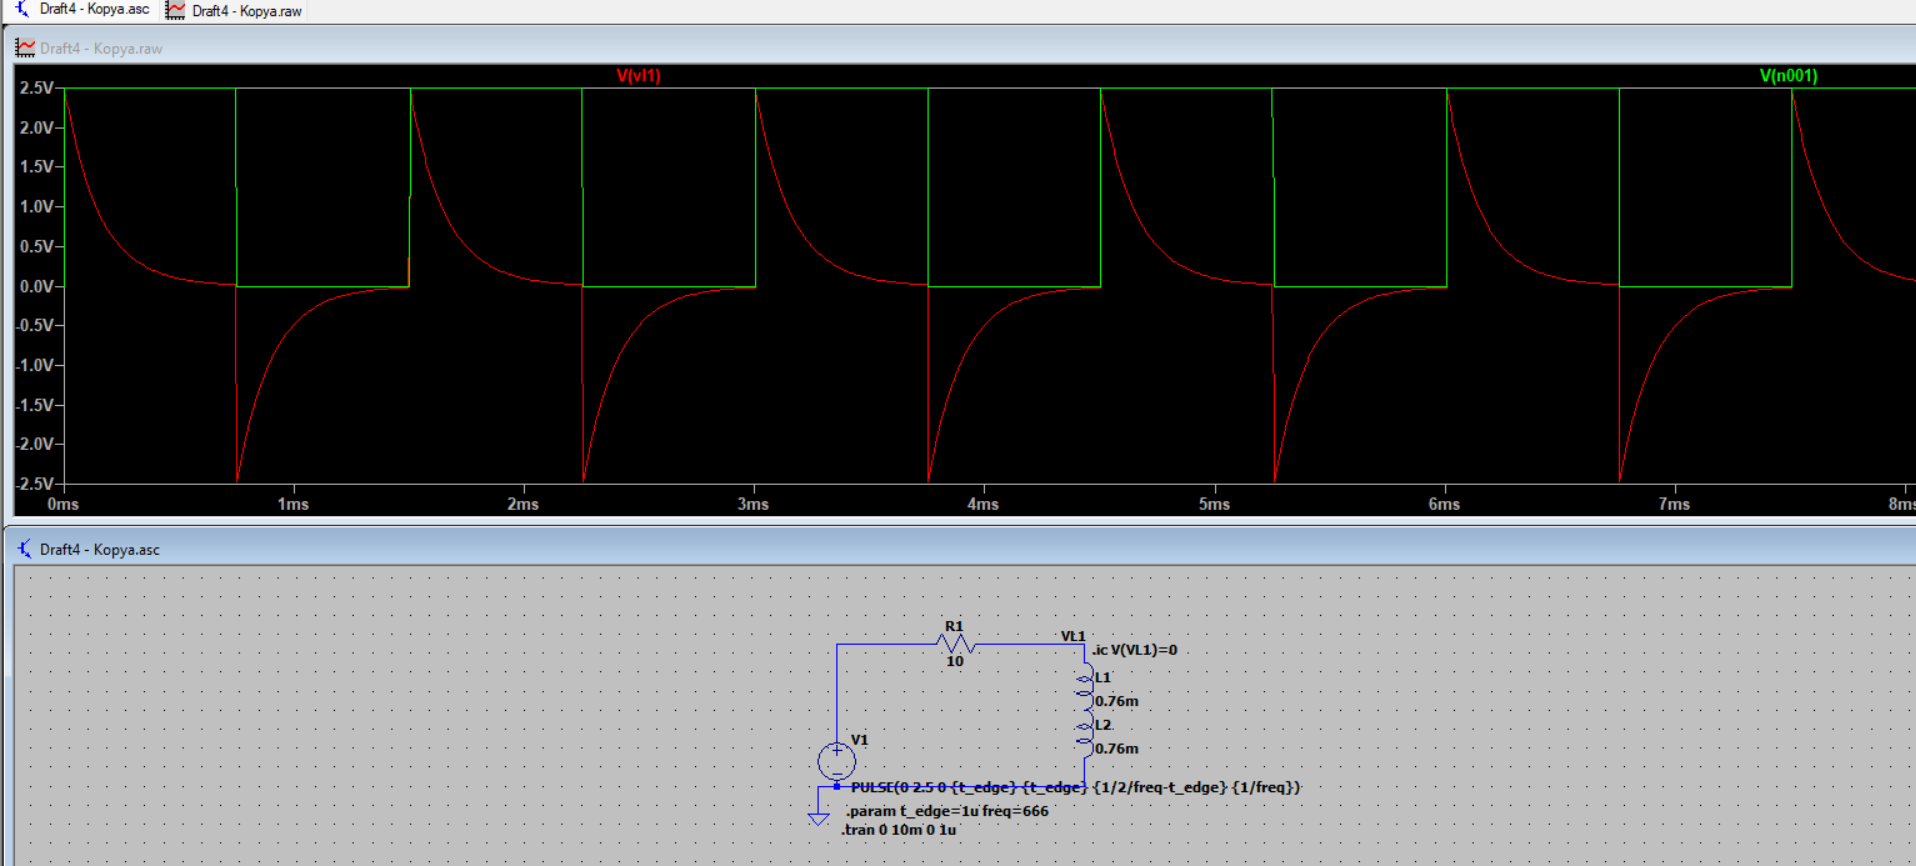
\includegraphics[width=1\textwidth]{assets/666-hz-2.5vpp-sim.png}
    \caption{666Hz Output @ $2.5V_{pp}$}
    \label{fig:666-hz-2.5vpp-output}
\end{figure}

Same characteristics as the experimental results are observed in the simulation.

\newpage{}
\thispagestyle{plain}

\subsubsection{T=L/R $\implies$ f=6.66kHz}

\begin{figure}[h]
    \centering
    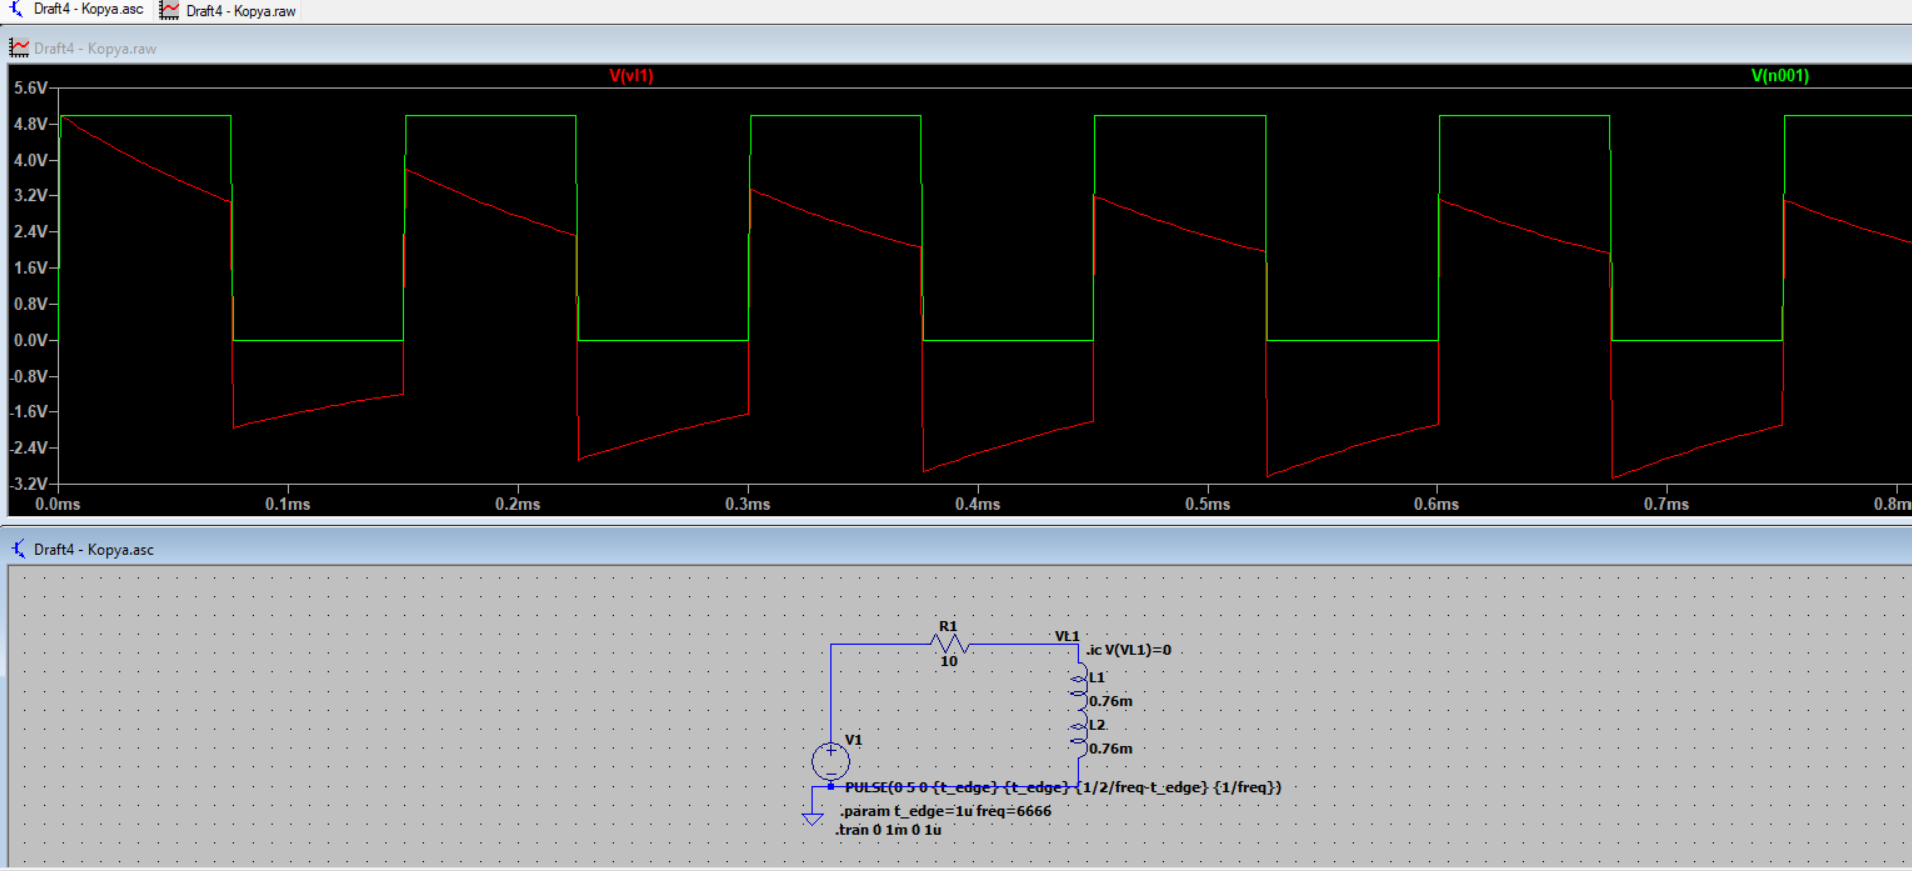
\includegraphics[width=1\textwidth]{assets/6666-hz-5vpp-sim.png}
    \caption{6.66kHz Output @ $5V_{pp}$}
    \label{fig:6666-hz-5vpp-output}
\end{figure}

\begin{figure}[h]
    \centering
    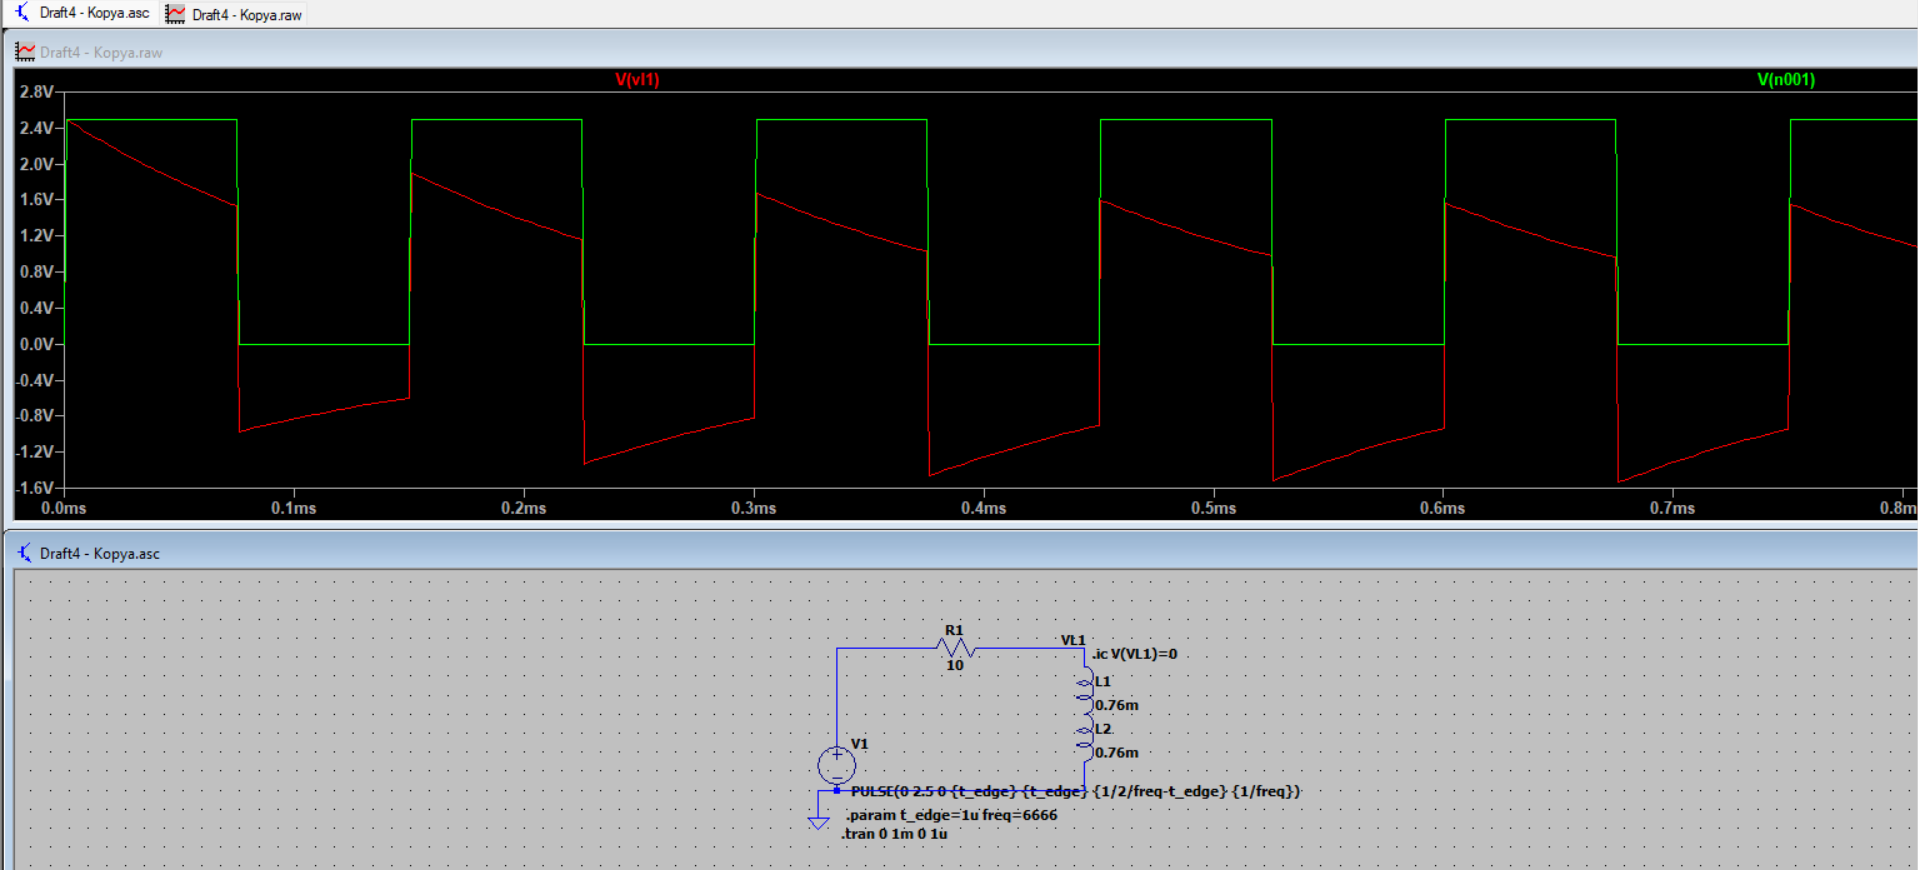
\includegraphics[width=1\textwidth]{assets/6666-hz-2.5vpp-sim.png}
    \caption{6.66kHz Output @ $2.5V_{pp}$}
    \label{fig:6666-hz-2.5vpp-output}
\end{figure}

Same characteristics as the experimental results are observed in the simulation.

\newpage{}
\thispagestyle{plain}

\subsubsection{T=L/10R $\implies$ f=66.66kHz}

\begin{figure}[h]
    \centering
    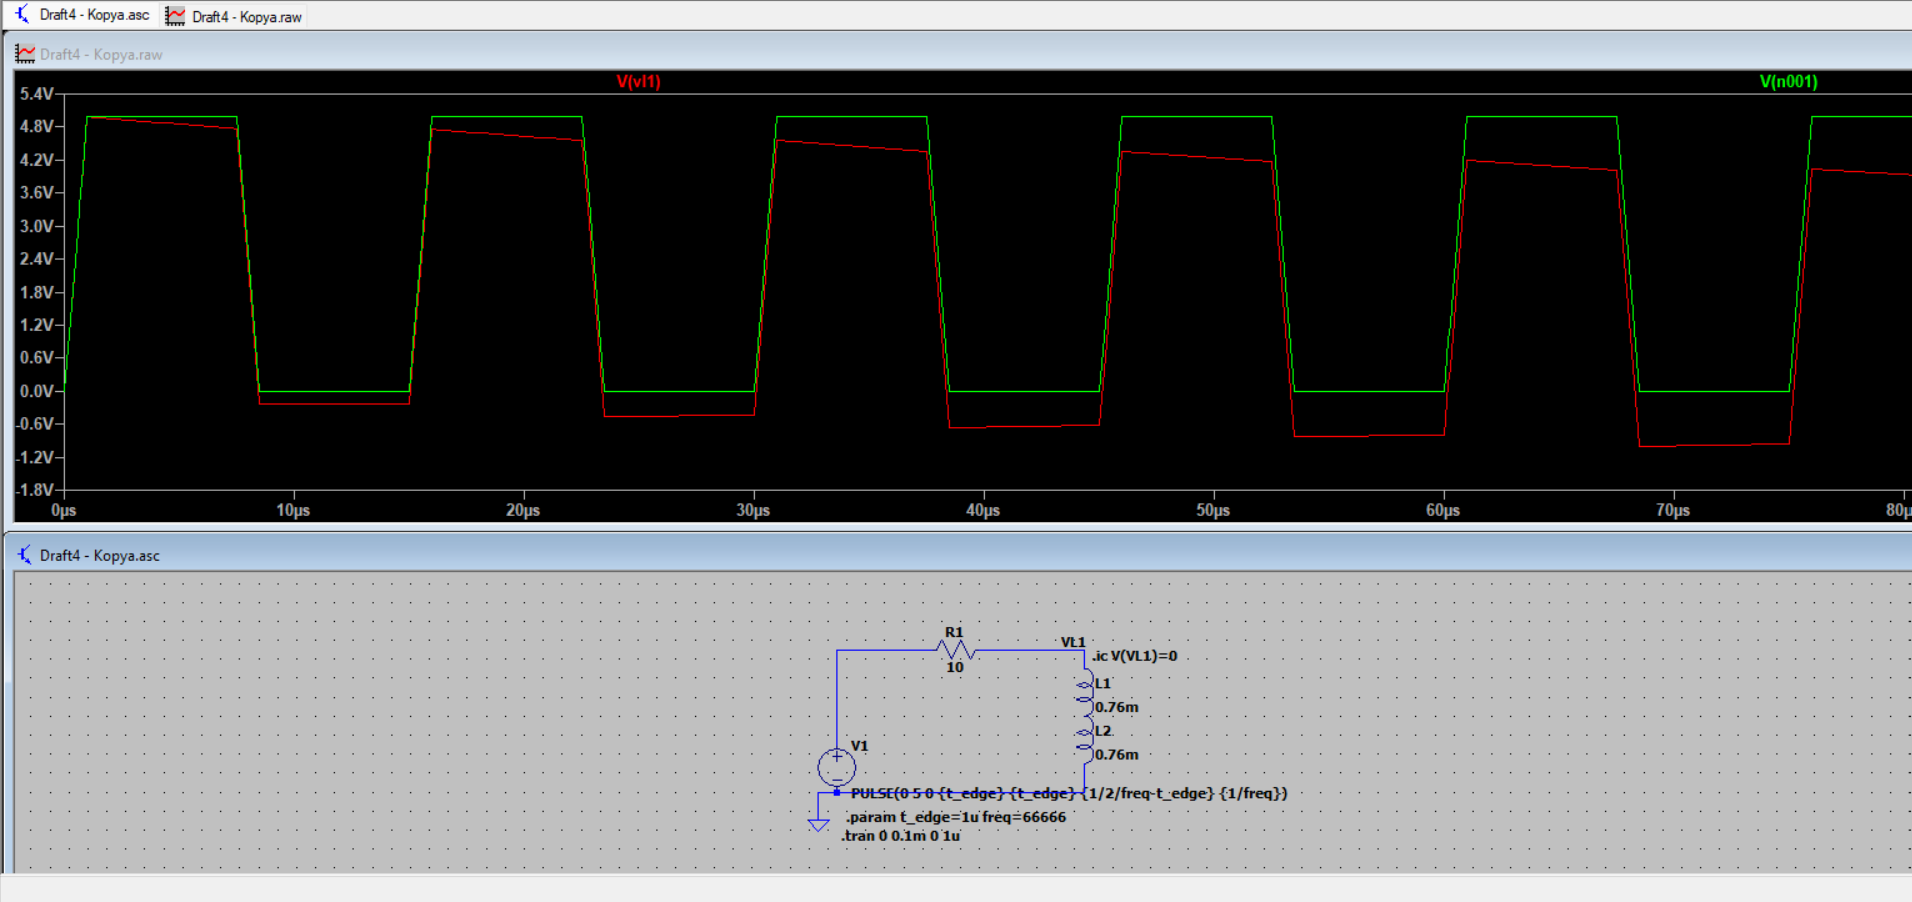
\includegraphics[width=1\textwidth]{assets/66666-hz-5vpp-sim.png}
    \caption{66.66kHz Output @ $5V_{pp}$}
    \label{fig:6666-hz-5vpp-output}
\end{figure}

\begin{figure}[h]
    \centering
    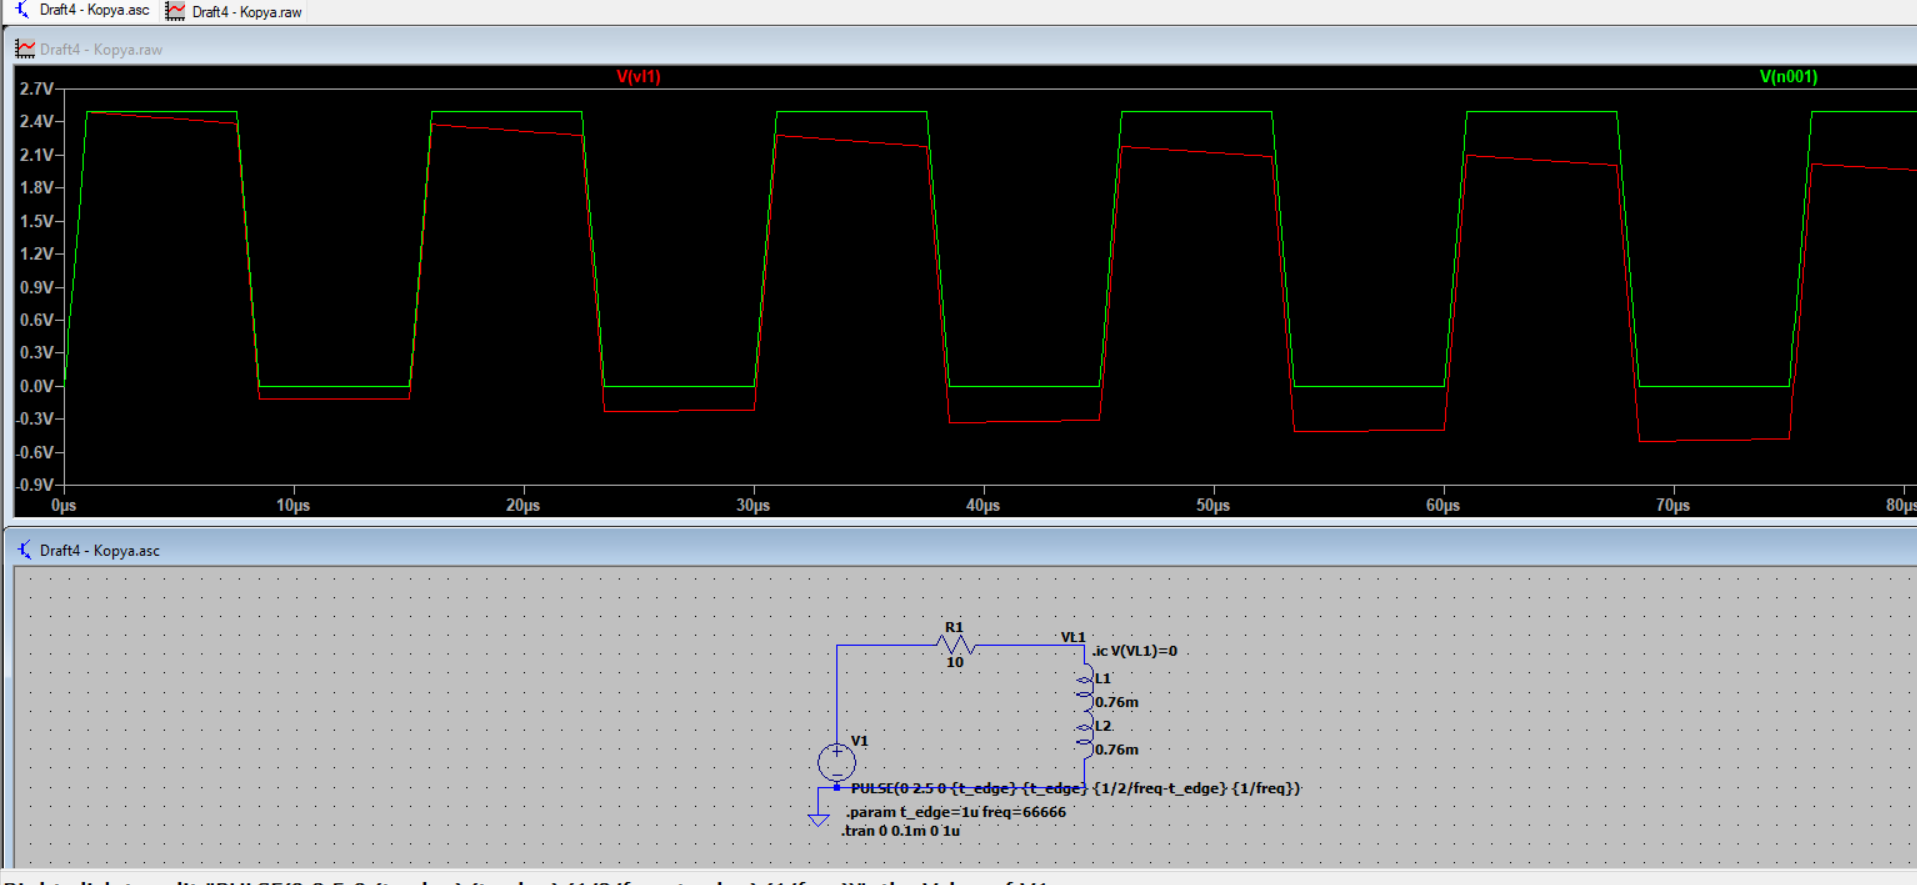
\includegraphics[width=1\textwidth]{assets/66666-hz-2.5vpp-sim.png}
    \caption{66.66kHz Output @ $2.5V_{pp}$}
    \label{fig:6666-hz-2.5vpp-output}
\end{figure}

Same characteristics as the experimental results are observed in the simulation.

\newpage{}
\thispagestyle{plain}

\subsubsection{Reducing the Amplitude}
When the amplitude of the square wave is reduced to half (0-2.5V), the voltages across both the inductor and the resistor also reduce proportionally. The overall behavior and response times remain consistent, but the magnitude of the voltages is halved.
